\documentclass{beamer}
\usepackage{amsmath}
\usepackage{tikz}
\usepackage{circle}
\usetheme{Boadilla}
\title[Alternating Automata]{Alternating Automata and Program Verification \nocite{Vardi::95}}
\date{April 11, 2012}

\author[Moshe Y. Vardi]{Moshe Y. Vardi}
\begin{document}
\setbeamercovered{transparent}

\AtBeginSection[]
{
    \begin{frame}{Table of Contents}
        \tableofcontents[currentsection]
    \end{frame}
}

\begin{frame}
\titlepage
\begin{center}
Presented by Ismail Badawi
\end{center}
\end{frame}

\begin{frame}{Table of Contents}
\tableofcontents
\end{frame}

\section{Refresher}

\begin{frame}{NBAs}
In class we discussed nondeterministic B\"{u}chi automata at some length.

A nondeterministic B\"{u}chi automaton (NBA) $\mathcal{A}$ is a tuple
$(S, \Sigma, \delta, S_0, F)$ where
    \begin{itemize}
    \item $S$ is a finite set of states
    \item $\Sigma$ is an alphabet
    \item $\delta: S \times \Sigma \rightarrow 2^S$ is a transition function
    \item $S_0 \subseteq S$ is a set of initial states, and
    \item $F \subseteq S$ is a set of \emph{accept} states
    \end{itemize}
An NBA accepts a word $\sigma \in \Sigma^\omega$ if it visits the accepting
set $F$ infinitely often while processing $\sigma$.
\end{frame}

\begin{frame}{LTL model checking}
For a transition system $TS$, and an LTL formula $\varphi$, we have
\begin{align*}
TS \models \varphi &\iff Traces(TS) \subseteq Words(\varphi) \\
&\iff Traces(TS) \cap Words(\varphi)^C = \varnothing \\
&\iff Traces(TS) \cap Words(\neg \varphi) = \varnothing
\end{align*}
\end{frame}

\begin{frame}{Model checking algorithm}
Given the transition system $TS$, and the LTL formula $\varphi$
\begin{itemize}
\item Construct an NBA $\mathcal{A}$ with $\mathcal{L}_\omega(\mathcal{A}) = Words(\neg \varphi)$
    \begin{itemize}
    \item First construct a GNBA, then convert to an NBA
    \item $2^{O(|\varphi|)}$ time and space
    \end{itemize}
\pause
\item Construct the product transition system $\mathcal{A} \oplus TS$
    \begin{itemize}
    \item $\mathcal{L}_\omega(\mathcal{A} \oplus TS) = \mathcal{L}_\omega(\mathcal{A}) \cap \mathcal{L}_\omega(TS)$
    \item Time and space $O(|TS||\mathcal{A}|) = O(|TS|\cdot2^{O(|\varphi|)})$
    \end{itemize}
\pause
\item Check if $\mathcal{L}_\omega(\mathcal{A} \oplus TS)$ is empty
    \begin{itemize}
    \item Linear time
    \end{itemize}
\pause
\item Total running time: $O(|TS|\cdot2^{O(|\varphi|)})$
\end{itemize}
\end{frame}
 
\section{Alternating Automata}
\begin{frame}{Towards ABAs}
\begin{itemize}
\item $\delta: S \times \Sigma \rightarrow 2^S$
\begin{itemize}
    \item e.g. $\delta(s, a) = \{s_1, s_2\}$
    \item i.e. if the automaton, from state $s$, reads a symbol $a$, it
    can move to state $s_1$, or to state $s_2$
\pause
    \item Some more suggestive notation... let us instead write
    $$ \delta(s, a) = s_1 \vee s_2 $$
\pause
    \item What would it mean to say
    $$ \delta(s, a) = s_1 \wedge s_2 $$
\end{itemize}
\end{itemize}
\end{frame}

\begin{frame}{Alternating B\"{u}chi Automata}
Alternating B\"{u}chi automata (ABAs) are defined just like NBAs, except 
that the transition function is
$$ \rho: S \times \Sigma \rightarrow \mathcal{B}^+(S)$$
where $\mathcal{B}^+(S)$ is the set of \emph{positive formulas over $S$}, i.e. boolean formulas built from
elements in $S$ using only disjunctions ($\vee$) and conjunctions ($\wedge$). (We also allow $true$ and $false$
as formulas.)
\end{frame}

\begin{frame}{Positive formulas}
\begin{itemize}
\item $\varphi = (s_1 \vee s_3) \wedge (s_2 \vee s_4) $
    \begin{itemize}
    \item We can think of $\varphi$ being satisfied by a set of states. \\
    \item $\{s_1, s_2\} \models \varphi$, but $\{s_1, s_3\} \not \models \varphi$
    \end{itemize}
\pause
\item $\rho(s, a) = \varphi$
    \begin{itemize}
    \item After reading symbol $a$ from state $s$, move to a set of states
    satisfying that formula
    \item Can be in multiple states at once!
    \item Another way to look at it: if $\sigma = aw$, the automaton accepts
    $\sigma$ from state $s$ if it accepts $w$ from $s_1$ or $s_3$ and from
    $s_2$ or $s_4$
    \end{itemize}
\end{itemize}
\end{frame}

\begin{frame}{Runs on ABAs}
\begin{itemize}
\item A run on an NBA was an infinite word over $\Sigma$.
\item For ABAs, runs are \emph{trees}, where every node is labeled with a state.
\item For every node, the set of states labeling its children must satisfy the transition formula.
\end{itemize}
\end{frame}

\begin{frame}{Example run}
Say we have $\Sigma = \{0, 1\}, Q = \{s_1, s_2\}$, $Q_0 = \{s_1\}$ and $\rho$ is defined by \\
\begin{center}
\begin{tabular}{| l | l | l |}
\hline & 0 & 1 \\ \hline
$s_1$ & $s_2$ & $s_1 \wedge s_2$ \\ \hline
$s_2$ & $s_1$ & $s_1 \vee s_2$ \\ \hline
\end{tabular}
\end{center}
Then (the start of) a run on input $0110...$ might look like \\
$$
\begin{tikzpicture}[auto]
\node (1) {$s_1$};
\node [right of=1] (2) {$s_2$};
\node [right of=2] (3) {$s_1$};
\node [above right of=3] (4a) {$s_1$};
\node [below right of=3] (4b) {$s_2$};
\node [right of=4a] (5a) {$s_2$};
\node [right of=4b] (5b) {$s_1$};
\node [right of=5a] (d1) {$\dots$};
\node [right of=5b] (d2) {$\dots$};
\path[->] (1) edge node {{\tiny $0$}} (2)
          (2) edge node {{\tiny $1$}} (3)
          (3) edge node {{\tiny $1$}} (4a)
          (3) edge node [below left] {{\tiny $1$}} (4b)
          (4a) edge node {{\tiny $0$}} (5a)
          (4b) edge node {{\tiny $0$}} (5b)
          (5a) edge node {} (d1)
          (5b) edge node {} (d2);
\end{tikzpicture}
$$
\end{frame}

\begin{frame}{Acceptance conditions}
\begin{itemize}
\item Note that a run might have finite branches; this can happen if we hit the $true$ or $false$ transitions.
\item A run is accepting if every \emph{infinite} branch hits the accept set infinitely often.
\item i.e. every branch either hits the $true$ transition, or hits the accept set infinitely often.
\end{itemize}
\end{frame}

\section{Translating LTL formulas to ABAs}
\begin{frame}{LTL}
$$ \varphi ::= 
true \mid a \mid \varphi_1 \wedge \varphi_2 \mid \neg \varphi \mid \Circle \varphi \mid \varphi_1 U \varphi_2
$$
For $\sigma = A_0A_1A_2\dots \in (2^{AP})^\omega$, we have
\begin{alignat*}{3}
\sigma &\models true & \\
\sigma &\models a &\iff& a \in A_0 \\
\sigma &\models \varphi_1 \wedge \varphi_2 &\iff& \sigma \models \varphi_1 \text{ and } \sigma \models \varphi_2 \\
\sigma &\models \neg \varphi &\iff& \sigma \not \models \varphi \\
\sigma &\models \Circle \varphi &\iff& \sigma[1\dots] \models \varphi \\
\sigma &\models \varphi_1 U \varphi_2 &\iff& \exists j \geq 0. \sigma[j\dots] \models \varphi_2 \text{ and } \sigma[i\dots] \models \varphi_1, \forall 0 \leq i < j \\
\end{alignat*}
(Nothing new here.)
\end{frame}

\begin{frame}{The ABA}
Given an LTL formula $\varphi$, let $\mathcal{A}_\varphi = (S, \Sigma, \rho, s_0, F)$, where
\begin{itemize}
\item $\Sigma$ is $2^{AP}$
\item $S$ is the set of all subformulas of $\varphi$, and their negation
    \begin{itemize}
    \item Idea: $\sigma \models s \iff \mathcal{A}_\varphi$ accepts $\sigma$ from state $s$
    \item This implies $s_0$ is $\varphi$ itself
    \end{itemize}
\item $F$ is the set of all formulas of the form $\neg (\varphi_1 U \varphi_2)$
\end{itemize}
\end{frame}

\begin{frame}{The transition function}
$$\rho: S \times \Sigma: \mathcal{B}^+(S)$$
\begin{align*}
\rho(p, a) &= true \qquad \text{if }  p \in a \\
\rho(p, a) &= false \qquad \text{if } p \not \in a \\
\rho(\varphi_1 \wedge \varphi_2, a) &= \rho(\varphi_1, a) \wedge \rho(\varphi_2, a) \\
\rho(\neg \varphi, a) &= \overline{\rho(\varphi, a)} \\
\rho(\Circle \psi, a) &= \psi \\
\rho(\varphi_1 U \varphi_2, a) &= \rho(\varphi_2, a) \vee (\rho(\varphi_1, a) \wedge \varphi_1 U \varphi_2)
\end{align*}
\end{frame}

\begin{frame}{Examples (1)}
$$AP = \{p, q\} \qquad \varphi = \Circle \Circle p \wedge q \qquad \sigma = \varnothing \varnothing \{p, q\} \dots$$
$$
\begin{tikzpicture}[node distance=5em, auto]
\node (1) {$\Circle \Circle p \wedge q$};
\node [right of=1] (2) {$\Circle p \wedge q$};
\node [right of=2] (3) {$p \wedge q$};
\node [above right of=3] (4a) {};
\node [below right of=3] (4b) {};
\path[->] (1) edge node {{\tiny $\varnothing$}} (2)
          (2) edge node {{\tiny $\varnothing$}} (3)
          (3) edge node {{\tiny $\{p, q\}$}} (4a)
          (3) edge node [below left] {{\tiny $\{p, q\}$}} (4b);
\end{tikzpicture}
$$
\end{frame}

\begin{frame}{Examples (2)}
$$AP = \{p, q\} \qquad \varphi = p U q \qquad \sigma = \{p\} \{p\} \{q\} \dots$$
$$
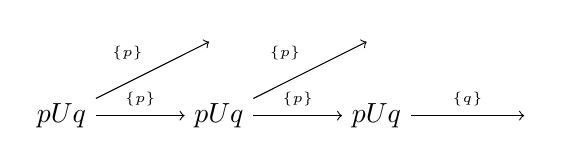
\begin{tikzpicture}[node distance=5em, auto]
\node (1) at (0, 0) {$p U q$};
\node (2a) at (2, 1) {};
\node (2) at (2, 0) {$p U q$};
\node (3a) at (4, 1) {};
\node (3) at (4, 0) {$p U q$};
\node (4) at (6, 0) {};
\path[->] (1) edge node {{\tiny $\{p\}$}} (2a)
          (1) edge node {{\tiny $\{p\}$}} (2)
          (2) edge node {{\tiny $\{p\}$}} (3a)
          (2) edge node {{\tiny $\{p\}$}} (3)
          (3) edge node {{\tiny $\{q\}$}} (4);
\end{tikzpicture}
$$
\end{frame}

\begin{frame}{Infinite runs?}
\begin{itemize}
\item In the previous two examples the accepting runs were finite, i.e. we
always hit the $true$ transition in every branch.
\item Actually there is only one kind of formula where the accepting runs
are infinite; formulas of the form $\neg (\varphi_1 U \varphi_2)$.
    \begin{itemize}
    \item Recall this is how we defined $\Box \varphi$, namely as $\neg (true \, U \neg \varphi)$
    \end{itemize}
\end{itemize}
\end{frame}

\begin{frame}{Examples (3)}
$$AP = \{p, q\} \qquad \varphi = \Box p = \neg (true \, U \neg p) \qquad \sigma = \{p\} \{p\} \{p\} \dots$$
\begin{align*}
\rho(\neg (true \, U \neg p), a) &= \overline{\rho(\neg p, a) \vee ((\rho(true, a) \wedge true \, U \neg p)} \\
&= \overline{\rho(\neg p, a)} \wedge \overline{true \, U \neg p} \\
&= \rho(p, a) \wedge \neg (true \, U \neg p)
\end{align*}
$$
\begin{tikzpicture}[node distance=5em, auto]
\node (1) at (0, 0) {$\Box p$};
\node (2a) at (2, 1) {};
\node (2) at (2, 0) {$\Box p$};
\node (3a) at (4, 1) {};
\node (3) at (4, 0) {$\Box p$};
\node (5a) at (6, 1) {};
\node (4) at (6, 0) {$\Box p$};
\node (5) at (8, 0) {$\dots$};
\path[->] (1) edge node {{\tiny $\{p\}$}} (2a)
          (1) edge node {{\tiny $\{p\}$}} (2)
          (2) edge node {{\tiny $\{p\}$}} (3a)
          (2) edge node {{\tiny $\{p\}$}} (3)
          (3) edge node {{\tiny $\{p\}$}} (5a)
          (3) edge node {{\tiny $\{p\}$}} (4)
          (4) edge node {{\tiny $\{p\}$}} (5);
\end{tikzpicture}
$$                                          
\end{frame}

\begin{frame}{Great?}
\begin{itemize}
\item So this is nice; $\mathcal{A}_\varphi$ has $O(|\varphi|)$ states.
    \begin{itemize}
    \item The translation takes \emph{linear} time and space, whereas 
          constructing an NBA took exponential time and space!
    \end{itemize}
\pause
\item However it turns out nonemptiness checking for a general ABA is not
really straightforward.
    \begin{itemize}
    \item The algorithm presented in the paper is to convert to an NBA
          (exponential blowup) then do the nonemptiness check there.
    \end{itemize}
\pause
\item So the LTL model checking algorithm that results from this is no
better than what we saw in class: $O(|TS| \cdot 2^{O(|\varphi|)})$.
\end{itemize}
\end{frame}

\begin{frame}{CTL Model Checking}
\begin{itemize}
\item In class the approach we saw for model checking CTL was not based on
automata theory.
\pause
\item Actually there are are automata-theoretic approaches to CTL model
checking; they use automata that operate on trees instead of words. 
    \begin{itemize}
    \item Similar sort of approach where, given a CTL formula $\varphi$, we 
    construct an automaton accepting exactly the programs satisfying $\varphi$
    \end{itemize}
\pause
\item But as in NBAs on words, translating a CTL formula to an NBA has
an exponential blowup. 
    \begin{itemize}
    \item This is bad because as we saw, CTL model checking can done in linear time, i.e.  $O(|TS||\varphi|)$.  
    \end{itemize}
\pause
\item Alternating B\"{u}chi automata on trees, using the same idea as we've
seen here, take linear time to construct.
\pause
\item The automata that arise from CTL formulas have a special structure to
them, so that we can do nonemptiness checking in linear time, without
first converting to an NBA.
\end{itemize}
\end{frame}

\begin{frame}{Summary}
\begin{itemize}
\item Alternating automata are a generalization of nondetermistic B\"{u}chi
automata, which have the power of universal choice in addition to
existential choice (as in plain nondeterminism).
\item They are equivalent in power to NBAs, but a lot more succinct/expressive.
\item There are nice straightforward translations from temporal logic
formulas to alternating automata, which can be done in linear time (i.e.
no exponential blowup as in NBAs).
\item This is nice because it allows us to use the same approach for
model checking both LTL and CTL.
\end{itemize}
\end{frame}

\begin{frame}{References}
\bibliographystyle{plain}
{\footnotesize
\bibliography{bib}}
\end{frame}
\end{document}
